\setcounter{chapter}{12}

\chapter{幂级数与Fourier级数}

\section{幂级数及其应用}

\subsection{函数项级数的概念}

{\bf 数项级数(无穷级数):}无穷多个{\it 数值}依序相加
$$S=\sum\limits_{n=1}^{\infty}u_n
=\lim\limits_{n\to\infty}\sum\limits_{k=1}^nu_k$$ 

{\bf 函数项级数:} 无穷多个{\it 函数}依序相加 
$$S(x)=\sum\limits_{n=1}^{\infty}u_n(x)
=\lim\limits_{n\to\infty}\sum\limits_{k=1}^nu_k(x)$$

{\bf 幂级数:} 
$$S(x)=\sum\limits_{n=0}^{\infty}a_n(x-x_0)^n$$ 

{\bf Fourier级数:} 
$$S(x)=\df{a_0}{2}+\sum\limits_{n=1}^{\infty}
(a_n\cos nx+b_n\sin nx)$$

\subsection{幂级数的概念与性质}

$${S(x)=\sum\limits_{n=0}^{\infty}a_n(x-x_0)^n}$$
其中:$a_n\in\mathbb{R}\,(n\in\mathbb{N})$,$x,x_0\in\mathbb{R}$。我们以
$${S(x)=\sum\limits_{n=0}^{\infty}a_nx^n}$$
为代表研究幂级数的有关性质。

\subsubsection{收敛性}

\begin{enumerate}[(1)]
  \setlength{\itemindent}{1cm}
  \item $\sum\limits_{n=0}^{\infty}\df{x^n}{n!}$\hfill $(-\infty<x<+\infty)$
  \item $\sum\limits_{n=0}^{\infty}x^n$\hfill $(|x|<1)$
  \item $\sum\limits_{n=0}^{\infty}n!x^n$ \hfill $x=0)$
\end{enumerate}

{\bf 注:}幂级数总是在某个区间上收敛或者发散,且其收敛的区域非空,具有对称性。

{\bf 定理13.1.1}(Abel定理)考虑幂级数
$$\sum\limits_{n=0}^{\infty}a_nx^n$$
\begin{enumerate}[(1)]
  \setlength{\itemindent}{1cm}
  \item 若在$x_0\ne 0$处该级数收敛,则对任意$|x|<|x_0|$,该级数绝对收敛; 
  \item 若在$x_0\ne 0$处该级数发散,则对任意$|x|>|x_0|$,该级数发散。 
\end{enumerate}

{\bf 推论:}存在收敛与发散的临界点:$x^*=\pm R$,使得幂级数在
以$x_0$为中心$R$为半径({\it 收敛半径})的对称区间内收敛,在其外发散。

{\bf 注:}在临界点处的收敛性需要单独判定!

{\bf 例:}若级数$S(x)=\sum\limits_{n=0}^{\infty}a_n(x-x_0)^n$在$x_1$
处条件收敛,则\underline{$R=|x_1-x_0|$}

{\bf 定理13.1.3-4:}若$\sum\limits_{n=0}^{\infty}a_nx^n$的系数满足
$$\limn\left|\df{a_{n+1}}{a_n}\right|=\rho
\quad\mbox{或}\quad\limn\sqrt[n]{|a_n|}=\rho,$$
则$R=1/\rho$。

{\bf 例:}求下列幂级数的收敛域
\begin{enumerate}[(1)]
  \setlength{\itemindent}{1cm}
  \item $\sum\limits_{n=0}^{\infty}\df{2+(-1)^n}{2^n}x^n$
  \item $\sum\limits_{n=0}^{\infty}\df{(x-1)^n}{2^nn}$
  \item $\sum\limits_{n=0}^{\infty}2^nx^{2n}$
\end{enumerate}

{\bf 注:}求幂级数的收敛域:先求半径,再讨论端点

{\bf 讨论:}
\begin{enumerate}
  \setlength{\itemindent}{1cm}
  \item 标准型幂级数: $\sum\limits_{n=0}^{\infty}a_nx^n$ 
  $${R=\limn\left|\df{a_n}{a_{n+1}}\right|}
  \quad\mbox{或}\quad {R=\df 1{\limn\sqrt[n]{|a_n|}}}$$ 
  \item 非标准型幂级数(缺项或通项为复合函数)先换元、整理,再求收敛半径 
  \item 比值法极限不存在时,注意使用根值法
\end{enumerate}

\subsection{幂级数的和函数}

{\bf 定理3:}(幂级数的运算性质)
\begin{enumerate}
  \setlength{\itemindent}{1cm}
  \item 两个幂级数的和在其收敛域的交集内收敛
  \item 幂级数逐项求导或求不定积分后收敛半径不变; 
  \item 幂函数的和函数在其收敛域上连续; 
  \item 幂函数逐项求导或求不定积分后,对应和函数分别为原和函数的导函数和原函数。
\end{enumerate}

{\bf 例:}已知
$$\df{1}{x+1}=\sum\limits_{n=0}^{\infty}(-x)^n\;(|x|<1),$$
求幂级数
$$\sum\limits_{n=1}^{\infty}\df{(-1)^{n-1}}{n}x^n$$
的和函数。由此证明:
$$\ln 2=1-\df 12+\df 13-\df 14+\ldots+\df{(-1)^n}{n}+\ldots$$

{\bf 例:}求下列幂级数的和函数
\begin{enumerate}[(1)]
  \setlength{\itemindent}{1cm}
  \item $\sum\limits_{n=0}^{\infty}\df{x^n}{n!}$
  \item $\sum\limits_{n=0}^{\infty}nx^n$
  \item $\sum\limits_{n=0}^{\infty}\df{x^n}{n+1}$
  \item $\sum\limits_{n=0}^{\infty}n^2x^n$
\end{enumerate}

{\bf 例:}求数项级数$\sumn\sum\limits_{k=1}^n\df{k}{2^{n-1}}$的和。

\subsection{函数的幂级数展开}

函数$f(x)$在原点处的无穷阶Taylor展开式: 
$$f(x)=\sum\limits_{n=0}^{\infty}\df{f^{(n)}(0)}{n!}x^n$$
 称为:{\it $f(x)$在原点处的Taylor级数(Maclaurin级数)} 
 
{\bf 注:}展开的条件: $f(x)$在原点处无穷阶可导

\begin{enumerate}[(1)]
  \setlength{\itemindent}{1cm}
  \item $f(x)=1+x+4x^3-5x^{99}+x^{100}$ 
  \item $f(x)=(1-x)e^x$ 
  \item $f(x)=\sin(x-\pi/4)$ 
  \item $f(x)=\df 1{1-x^2}$ 
  \item $f(x)=\ln(2+x)$ 
  \item $f(x)=\arctan x$
\end{enumerate}

\subsection{幂级数的应用}

\subsubsection{函数值的近似计算}

\subsubsection{积分的近似计算}

\subsubsection{解微分方程}

{\bf 例:}求解初值问题:$$xy''+y'+xy=0,\;y(0)=1,\;y'(0)=0$$

\subsection{课堂练习}

{\bf 例:}判断正误
\begin{enumerate}[(1)]
  \setlength{\itemindent}{1cm}
  \item 幂级数在其收敛域上一定绝对收敛 \;{{$(\;\times\;)$}} 
  \item 设$\sum a_nx^n,\sum b_nx^n$的收敛半径分别为$R_1,R_2$,
  则$\sum(a_n+b_n)x^n$的收敛半径$R=\min\{R_1,R_2\}$ 
  \;{{$(\;\times\;)$}} 
  \item 幂级数与其逐项积分和逐项求导的幂级数的收敛域相同 
  \;{{$(\;\times\;)$}}
\end{enumerate}

{\bf 例:}若$\sum a_n(x-2)^n$在$x=-2$收敛,则在$x=5$处
\underline{\;{绝对收敛}\;};若在$x=-2$处条件收敛,
则收敛半径为\underline{\;{$4$}\;}

{\bf 例:}求函数项级数$\sum\limits_{n=1}^{\infty}
\sin\df 1 {3n}\left(\df{3+x}{3-2x}\right)^n$
的收敛域。

{\bf 例:}求级数$\sum\limits_{n=1}^{\infty}\df{n}{2^{n-1}}$的和。

{\bf 例:}将下列函数展开成Maclaurin级数,并求其收敛域
\begin{enumerate}[(1)]
  \setlength{\itemindent}{1cm}
  \item $f(x)=\arcsin x$
  \item $f(x)=\df 1{1+x+x^2}$
\end{enumerate}

\section{Fourier级数}

\subsection{三角级数与Fourier级数}

{\bf 函数的局部逼近}

$${f(x)=\sum\limits_{n=0}^{\infty}\df{f^{(n)}(x_0)}{n!}(x-x_0)^n}$$
\begin{center}
	\resizebox{!}{5cm}{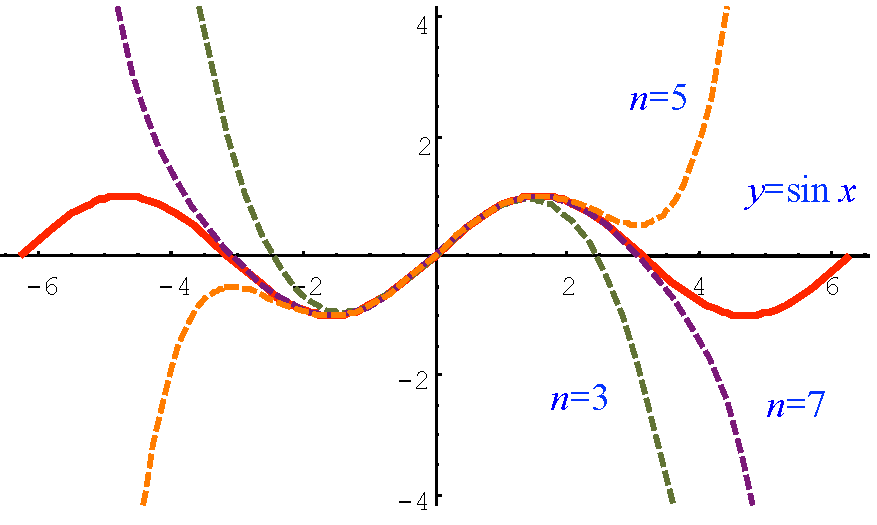
\includegraphics{./images/ch13/sinm.pdf}}
\end{center}

{\bf Insight:}利用周期运动来逼近周期运动会有更好的整体逼近效果!

{\bf 最简单的周期运动:}{\bb 简谐振动:} 例如弹簧振子、钟摆
$$f(t)=A\sin(\omega t+\varphi)$$
\begin{itemize} 
  \item { $A$:}振幅 
  \item { $\omega$:}角频率 
  \item { $\varphi$:}初相位 
\end{itemize}
记$x=\omega t,\,a=A\sin\varphi,\,b=A\cos\varphi$, 则
$${f(x)=a\cos x+b\sin x}$$

{\it Daniel Bernoulli (1700-1782):}任何复杂的振动都可以分解成一系列简谐振动之和

{\it Joseph Fourier (1768-1830):}“任意”函数都可以展开成三角级数

$${f(t)=A_0+\sumn A_n\sin(n\omega t+\varphi_n)}$$

{\bf 三角级数与周期函数的整体逼近}

$${f(x)=\df{\pi}{4}\mathrm{sgn}(x),\;(x\in[-\pi,\pi])
\;{\sim\;\sum\limits_{k=1}^n\df{\sin(2k-1)x}{2k-1}}}$$

\begin{center}
	\resizebox{!}{4cm}{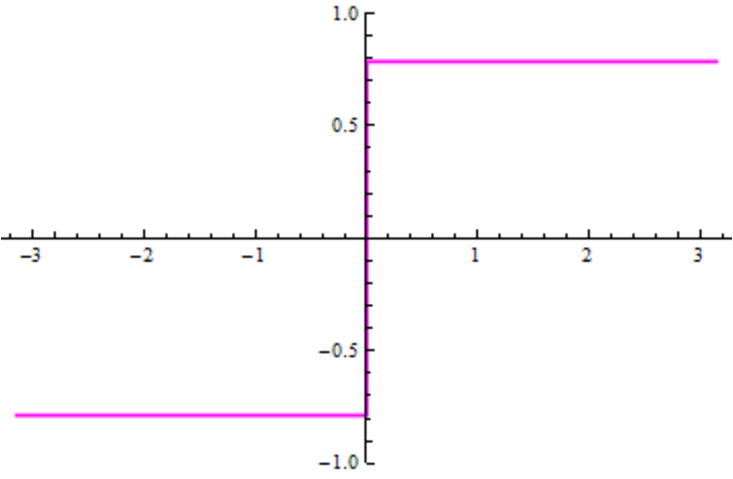
\includegraphics{./images/ch13/fsgn/f0.pdf}}
	\quad
	\resizebox{!}{4cm}{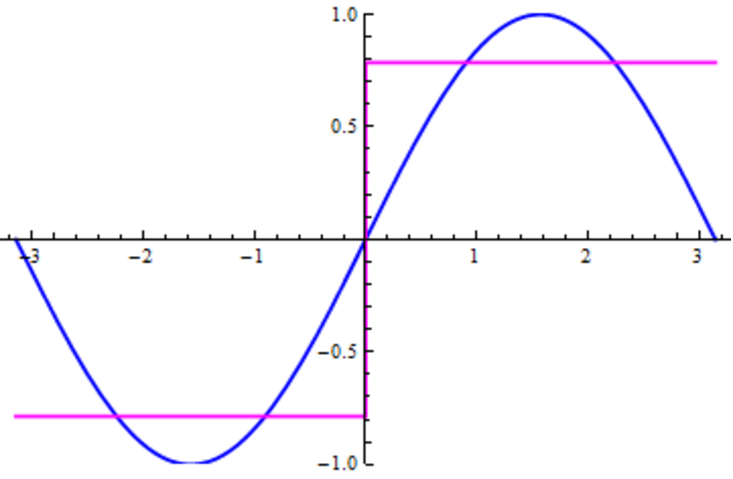
\includegraphics{./images/ch13/fsgn/f1.pdf}}
	
	\resizebox{!}{4cm}{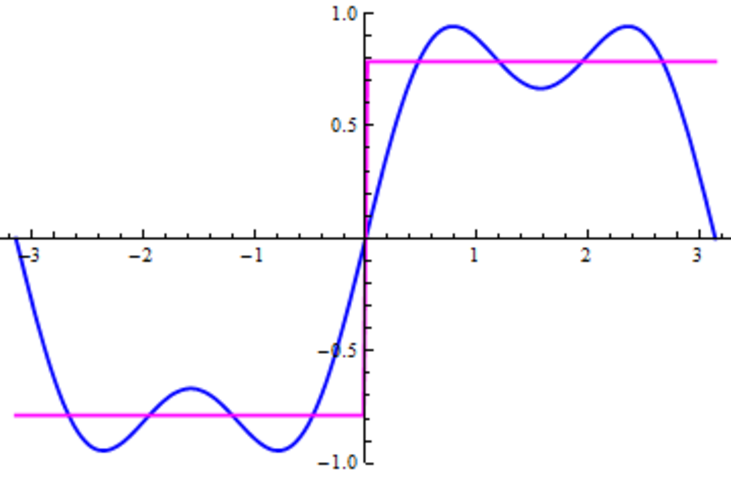
\includegraphics{./images/ch13/fsgn/f2.pdf}}
	\quad
	\resizebox{!}{4cm}{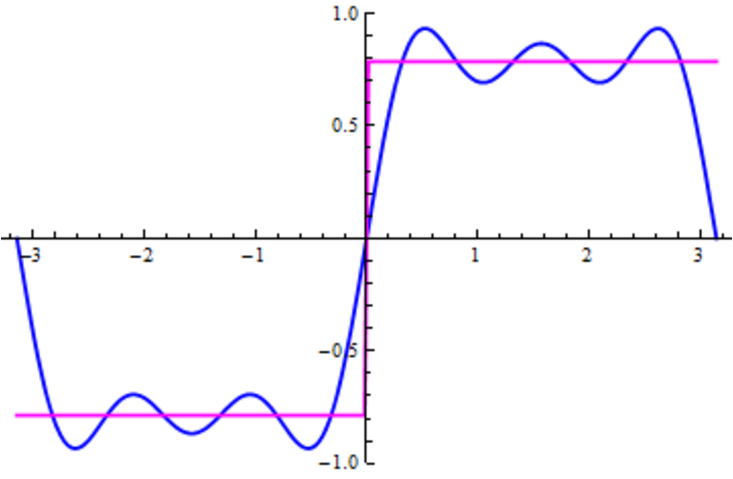
\includegraphics{./images/ch13/fsgn/f3.pdf}}
	
	\resizebox{!}{4cm}{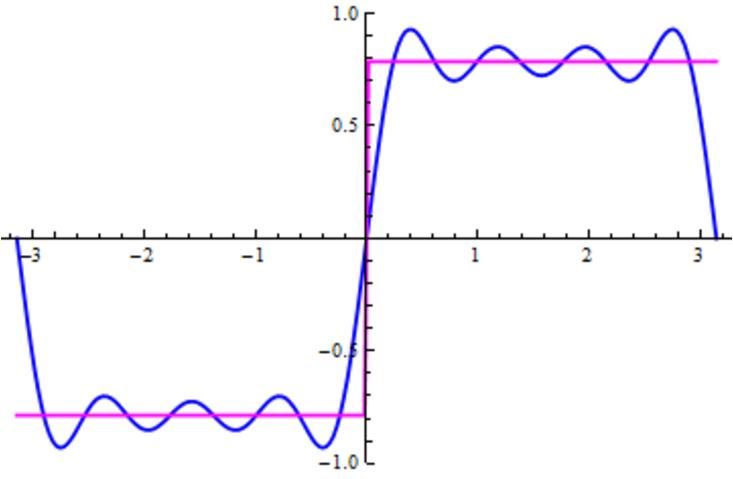
\includegraphics{./images/ch13/fsgn/f4.pdf}}
	\quad
	\resizebox{!}{4cm}{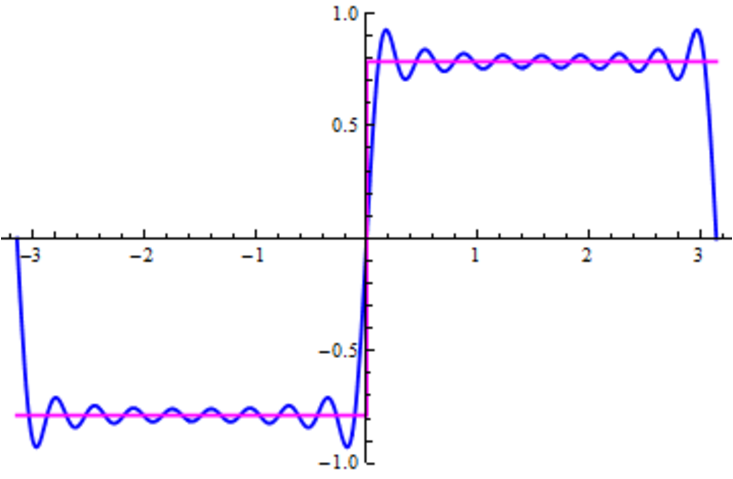
\includegraphics{./images/ch13/fsgn/f5.pdf}}
\end{center}

{\bf 三角级数}
$${\df{a_0}{2}+\sum\limits_{k=1}^{\infty}(a_k\cos kx
+b_k\sin kx)}$$ 

{\bf 性质:}
三角函数序列$A=\{\cos kx,\sin kx|k=1,2,\ldots\}$具有{\it 正交性} ,
即:任意$f(x),g(x)\in A$,
$$\dint_{-\pi}^{\pi}f(x)g(x)dx=\left\{\begin{array}{ll}
0,\;& f(x)\ne g(x)\\ \pi\;& f(x)=g(x)
\end{array}\right.$$

{\bf 定理:}若函数$f(x)$可展成如下三角级数
$$\df{a_0}{2}+\sum\limits_{k=1}^{\infty}(a_k\cos kx+b_k\sin kx),$$
且该三角级数可逐项积分, 则
$$\left\{\begin{array}{ll}
a_k=\df1{\pi}\dint_{-\pi}^{\pi}f(x)\cos kxdx,\;& k=0,1,2,\ldots\\[5pt]
b_k=\df1{\pi}\dint_{-\pi}^{\pi}f(x)\sin kxdx,\;& k=1,2,\ldots
\end{array}\right.$$

{\bf 注:}
\begin{enumerate}[(1)]
  \setlength{\itemindent}{1cm}
  \item $[-\pi,\pi]$上的奇函数的Fourier级数只含有正弦项, 称为{\it 正弦级数}
  $$\sum\limits_{k=1}^{n}b_k\sin kx$$ 
  \item $[-\pi,\pi]$上的偶函数的Fourier级数只含有余弦项, 称为{\it 余弦级数}
  $$\df{a_0}{2}+\sum\limits_{k=1}^{n}a_k\cos kx$$
\end{enumerate}

{\bf 例:}$f(x)$以$2\pi$为周期,且在$[-\pi,\pi]$内$f(x)=\df{\pi}{4}\mathrm{sgn}(x)$,
求其Fourier级数。

{\bf 例:}$f(x)$以$2\pi$为周期,且
$$f(x)=\left\{\begin{array}{rl}
	-\df{\pi}4,\;& -\pi\leq x<0\\[5pt]
	\df{\pi}4,\;& 0\leq x<\pi
\end{array}\right.$$
求其Fourier级数。

{\bf 注:}只在有限点处取值不同的函数,Fourier级数相同

{\bf 例:}$g(x)$以$2\pi$为周期,且
$$g(x)=\left\{\begin{array}{ll}
	0,\;& -\pi\leq x<0\\
	1,\;& 0\leq x<\pi
\end{array}\right.$$
求其Fourier级数。

{\bf 例:}将下列函数展成Fourier级数
\begin{enumerate}[(1)]
  \setlength{\itemindent}{1cm}
  \item $f(x)=1+3\sin x+4\cos 3x-9\sin 2x$
  \item $f(x)=\sin^4x$
\end{enumerate}

{\bf 注:}以$2\pi$为周期的三角多项式的Fourier级数是其自身

$${\df{a_0}{2}+\sum\limits_{k=1}^{n}(a_k\cos kx+b_k\sin kx)}$$

\subsection{Fourier级数的收敛性}

{\bf 定理13.2.1}(Dirichlet收敛条件)$f(x)$以$2\pi$为周期, 在$[-\pi,\pi]$上其
{\it 分段连续}且{\it 仅有有限多个极值点}, 则$f(x)$的Fourier级数在$[-\pi,\pi]$上收敛,
 其和函数
$$S(x) =\left\{\begin{array}{ll}
	\df{f(x+0)+f(x-0)}{2},\;& x\in(-\pi,\pi) \\[5pt]
	\df{f(-\pi+0)+f(\pi-0)}{2},\;& x=\pm\pi
\end{array}\right.$$

{\bf 注:}$S(x)$在$f(x)$的连续点处收敛于$f(x)$

{\bf 例:}试写出函数
$$f(x)=\left\{\begin{array}{rl}
	-\df{\pi}{4},\; & -\pi\leq x<0\\[8pt]
	\df{\pi}{4},\; & 0\leq x<\pi
\end{array}\right.$$
的Fourier级数的和函数。

$${S(x)=\left\{\begin{array}{ll}
	-\pi/4,\;& -\pi<x<0\\
	\pi/4,\;& 0<x<\pi\\
	0,\; & x=0,\pm\pi
\end{array}\right.}$$

{\bf 例:}设周期函数$f(x)$在一个周期内的表达式为
$$f(x)=\left\{\begin{array}{ll}
	-1,\;& -\pi<x\leq 0\\
	1+x^2,\; & 0<x\leq\pi
\end{array}\right.$$
写出该函数在$[-\pi,\pi]$上的和函数$S(x)$,并求
$S(5\pi/2),S(7\pi/2),S(7\pi)$和$S(2008\pi)$的值。

{\bf 利用Fourier级数求特殊级数的和}

{\bf 例:}由
$$\df{\pi}4=\sum\limits_{m=1}^{\infty}
\df{\sin(2m-1)x}{2m-1},\;0<x<\pi,$$
 令$x=\pi/2$, 可得
$$\df{\pi}4=1-\df 13+\df 15-\df 17+\ldots
+(-1)^{m-1}\df 1{2m-1}+\ldots$$

{\bf 例:}设$f(x)=|x|\;(-\pi\leq x\leq \pi)$的Fourier级数,并由此
证明:
$$\df{\pi^2}{6}=1+\df 1{2^2}+\df 1{3^2}+\ldots+\df 1{n^2}+\ldots$$
$${|x|=\df{\pi}2-\df 4{\pi}\sum\limits_{m=1}^{\infty} 
\df{\cos(2m-1)x}{(2m-1)^2},\;-\pi\leq x\leq \pi}$$

{\bf 例:}设周期函数$f(x)$在一个周期内的表达式为
$$f(x)=e^x\;(x\in[0,2\pi]),$$
试将其展成Fourier级数,并求下列数值级数的和:
$$\sum\limits_{n=1}^{\infty}\df1{1+n^2}$$

\subsection{函数的延拓及其Fourier展开}

{\bf 问:}如果函数$f(x)$只在$(0,\pi)$或$[0,\pi]$上有定义,能否/如何对其进行
Fourier展开?

{\bf 函数(定义)的延拓:} 扩充函数的定义域,使其具有某种期望的性质 
\begin{enumerate}[(1)]
  \setlength{\itemindent}{1cm}
  \item {\it 周期延拓:} 延拓后为周期函数 
  \item {\it 奇延拓:} 延拓后为奇函数 
  \item {\it 偶延拓:} 延拓后为偶函数
\end{enumerate}	

{\bf 周期延拓}

设$f(x)$在$(0,\pi)$上满足Dirichlet条件 
\begin{enumerate}[(1)]
  \setlength{\itemindent}{1cm}
  \item 任取在$[-\pi,0]$上满足Dirichlet条件的函数$g(x)$ 
  \item 令
  $$F(x)=\left\{\begin{array}{ll}
  	f(x),\;& x\in(0,\pi)\\
  	g(x),\;& x\in[-\pi,0]
  \end{array}\right.$$
   且
  $$F(x+2\pi)=F(x)\;(-\infty<x<\infty)$$
\end{enumerate}
$F(x)$为$(-\infty,\infty)$上满足Dirichlet条件的周期函数,
其在$(0,\pi)$上$f(x)$有相同的Fourier展开式

{\bf 奇(性)延拓}

设$f(x)$在$(0,\pi)$上满足Dirichlet条件 
\begin{itemize}
  \item 令
  $$F(x)=\left\{\begin{array}{ll}
  	f(x),\;& x\in(0,\pi)\\
  	0,\;& x=0,-\pi\\
  	-f(-x),\;& x\in(-\pi,0)
  \end{array}\right.$$
   且
  $$F(x+2\pi)=F(x)\;(-\infty<x<\infty)$$
\end{itemize}
$F(x)$为满足Dirichlet条件的奇周期函数,其Fourier级数为正弦级数,且
在$(0,\pi)$内与$f(x)$的展式相同

{\bf 偶(性)延拓}

设$f(x)$在$[0,\pi]$上满足Dirichlet条件 
\begin{itemize}
  \item 令
  $$F(x)=\left\{\begin{array}{ll}
  	f(x),\;& x\in[0,\pi]\\
  	f(-x),\;& x\in[-\pi,0)
  \end{array}\right.$$
   且
  $$F(x+2\pi)=F(x)\;(-\infty<x<\infty)$$
\end{itemize}
$F(x)$为满足Dirichlet条件的偶周期函数,其Fourier级数为余弦级数,且
在$(0,\pi)$内与$f(x)$的展式相同

{\bf 例:}设函数$f(x)=x+1\,(x\in(0,\pi))$,试将其分别展开为正弦和余弦级数。

\begin{center}
	\resizebox{!}{2.7cm}{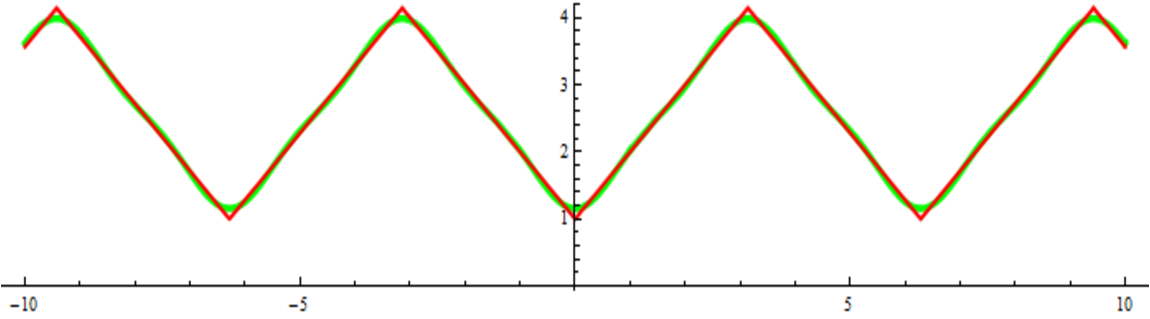
\includegraphics{./images/ch13/cs.pdf}} 
	
	\resizebox{!}{2.7cm}{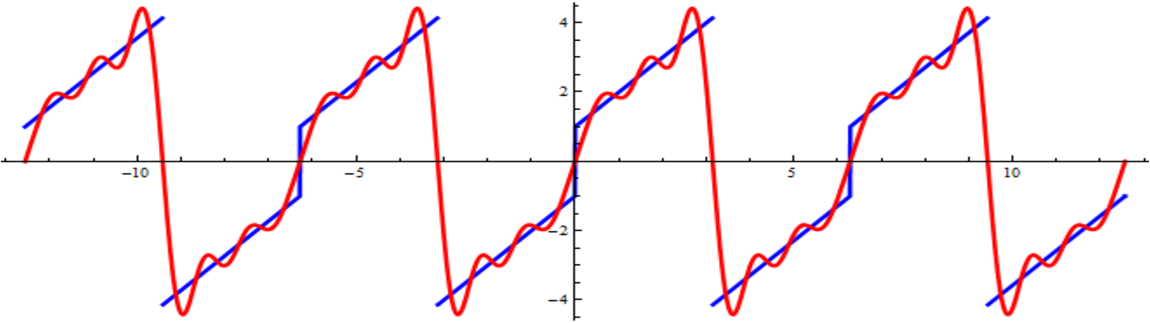
\includegraphics{./images/ch13/ss.pdf}}
\end{center}

{\bf 例:}设$f(x)=\pi x-x^2\,(0<x<\pi)$,又设$S(x)$是$f(x)$在$(0,\pi)$内以
$2\pi$为周期的正弦级数展开式的和函数,求当$x\in(\pi,2\pi)$时$S(x)$的表达式。

\subsection{周期为$2l$的Fourier级数}

{\bf 问:}对周期为$2l\ne2\pi$的函数$f(x)$,能否/如何将其展开为Fourier级数?

{\it 伸缩变换:} 令$t=\df{\pi}{l}x$,
则$g(t)=f\left(\df{l}{\pi}t\right)$ 是以$2\pi$为周期的函数。 
对$g(t)$做Fourier展开,由其展开式可变换得到$f(x)$的展开式。

{\bf 例:}将函数$f(x)=x\,(0<x<1)$表示为只有余弦项的三角级数。

\subsection{课堂练习}

{\bf 例:}判断正误
\begin{enumerate}[(1)]
  \setlength{\itemindent}{1cm}
  \item 函数$f(x)$连续,在$[-\pi,\pi]$上满足Dirichlet条件且为奇函数,则$f(x)$
  的Fourier级数在$0,\pm\pi$处必收敛于$0$\quad  (\;{$\surd$}\;) 
  \item $f(x)=x^2\,(x\in[-\pi,\pi])$的Fourier级数在$2\pi$处收敛于$4\pi^2$
    \quad(\;{$\times$}\;) 
  \item 以$2\pi$为周期的函数$f(x)=\df x{2\pi}\,(x\in[0,2\pi])$,其Fourier
  级数的和函数为$S(x)$,则$S(0)=f(0)=0$ 
  \quad (\;{$\times$}\;)
  \item 函数$f(x)=x^2\,(x\in[-\pi,\pi])$以$2\pi$为周期,则 
  \begin{itemize}
    \item $\df 1{\pi}\dint_{-\pi}^{\pi}f(x)\sin kxdx=\df
    1{\pi}\dint_{0}^{2\pi}f(x)\sin kxdx$\quad (\;{$\surd$}\;) 
    \item $\df 1{\pi}\dint_{-\pi}^{\pi}x^2\sin kxdx=\df
    1{\pi}\dint_{0}^{2\pi}x^2\sin kxdx$\quad (\;{$\times$}\;) 
  \end{itemize}
  \item 以$2\pi$为周期的函数$f(x)=x^2\,(x\in[-\pi,\pi])$和$g(x)=x^2\,(x\in[0,2\pi])$的
  Fourier级数相同\quad (\;{$\times$}\;)
\end{enumerate}

{\bf 例:}将下列函数展成Fourier级数
\begin{enumerate}[(1)]
  \setlength{\itemindent}{1cm}
  \item $f(x)=\sin^4x$
  \item $f(x)=\arcsin(\sin x)$
\end{enumerate}

{\bf 例:}设$f(x)$是以$2\pi$为周期的连续函数,在$[-\pi,\pi]$上满足Dirichlet条件,
且其Fourier系数为$a_k,b_k$。设
$$G(x)=\df1{\pi}\dint_{-\pi}^{\pi}f(t)f(x+t)dt$$
\begin{enumerate}[(1)]
  \setlength{\itemindent}{1cm}
  \item 证明$G(x)$为偶函数
  \item 求$G(x)$的Fourier系数
  \item 证明$\df1{\pi}\dint_{-\pi}^{\pi}f^2(x)dx=\df{a_0^2}2+
  \sum\limits_{k=1}^{\infty}(a_k^2+b_k^2)$
\end{enumerate}

\newpage

\section*{课后作业}

{\bf 【基本题】}

\begin{itemize}
  \setlength{\itemindent}{1cm}
  \item 习题13.1:2,8,17
  \item 习题13.2:1(1,4),3(1)
\end{itemize}

{\bf 【上交题】}

\begin{itemize}
  \setlength{\itemindent}{1cm}
  \item 习题13.1:3,6,14,20
  \item 习题13.2:5,8,9
\end{itemize}

{\bf 【思考题】}

\begin{itemize}
  \setlength{\itemindent}{1cm}
  \item 习题13.1:9,11,12,13,15,16,18,25,26
  \item 习题13.2:11,12,13
\end{itemize}